\chapter{General Addenda}

If there are several additions you want to add, but they do not fit into the thesis itself, they belong here.

\section{Detailed Addition}

Even sections are possible, but usually only used for several elements in, e.g.\ tables, images, etc.
\chapter{Appendix}
\begin{figure}
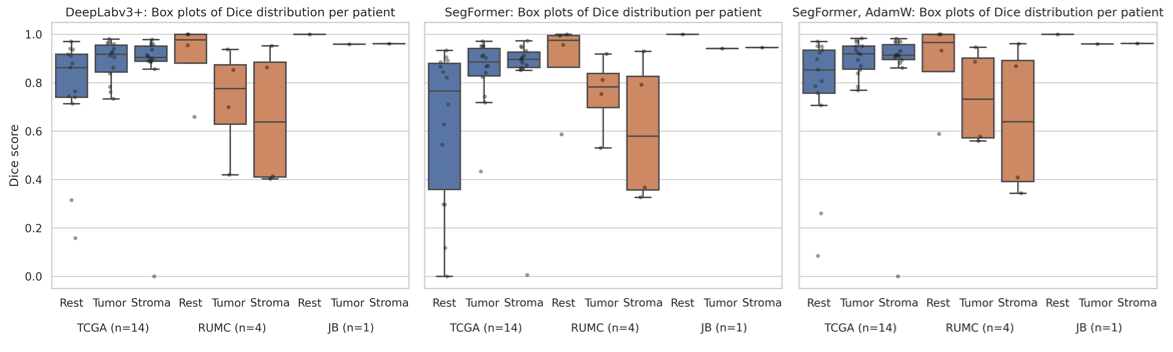
\includegraphics[width=\linewidth]{figures/tissue/dices_patients.png}
\caption{EXAMPLES for TILs prediction models. A lot of test comming up here.}
\label{fig:figure3}
\end{figure}

\begin{figure}
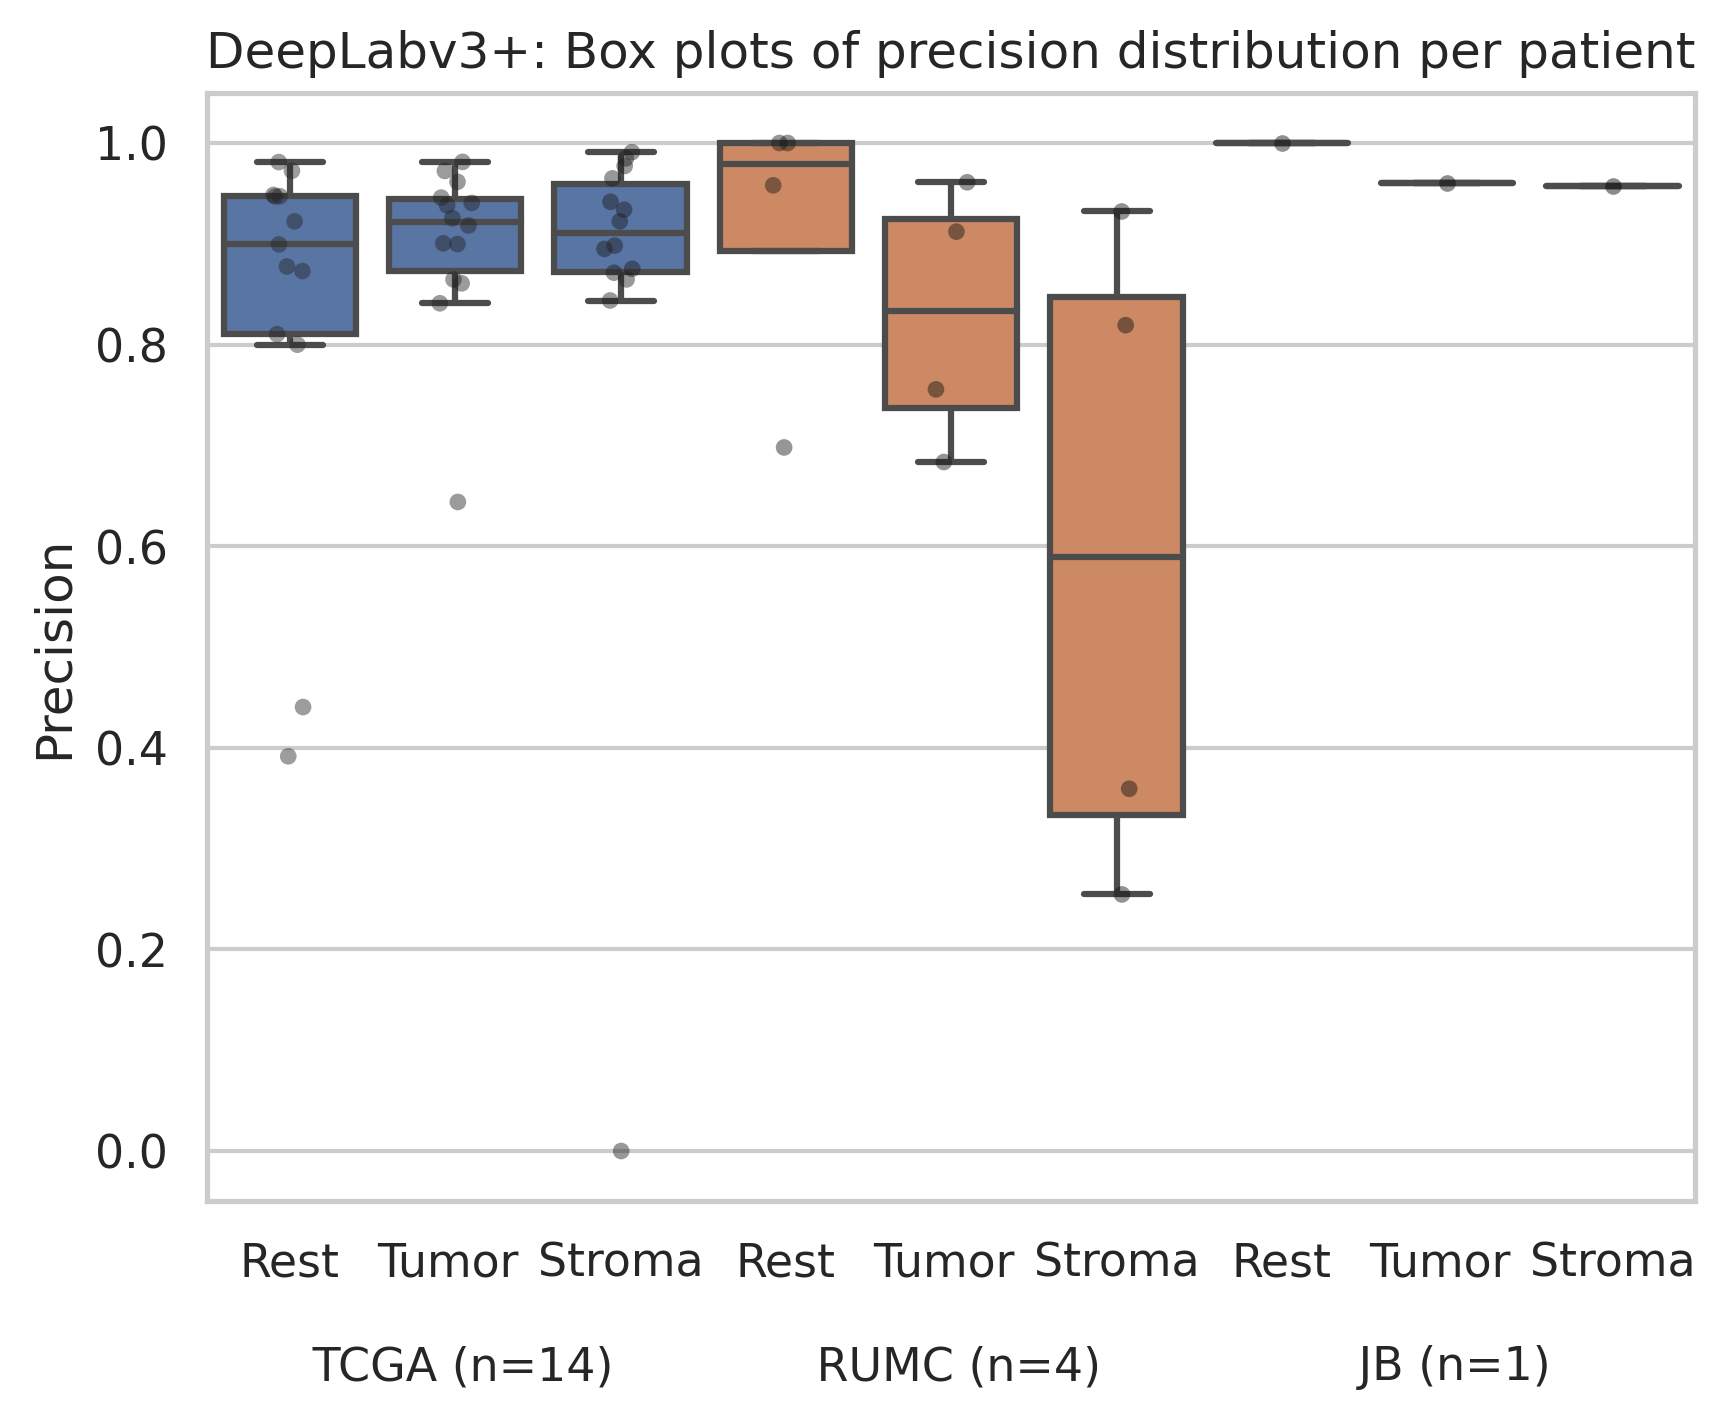
\includegraphics[width=.5\linewidth]{figures/tissue/deeplabv3+_prec_patient_wsirois.png}
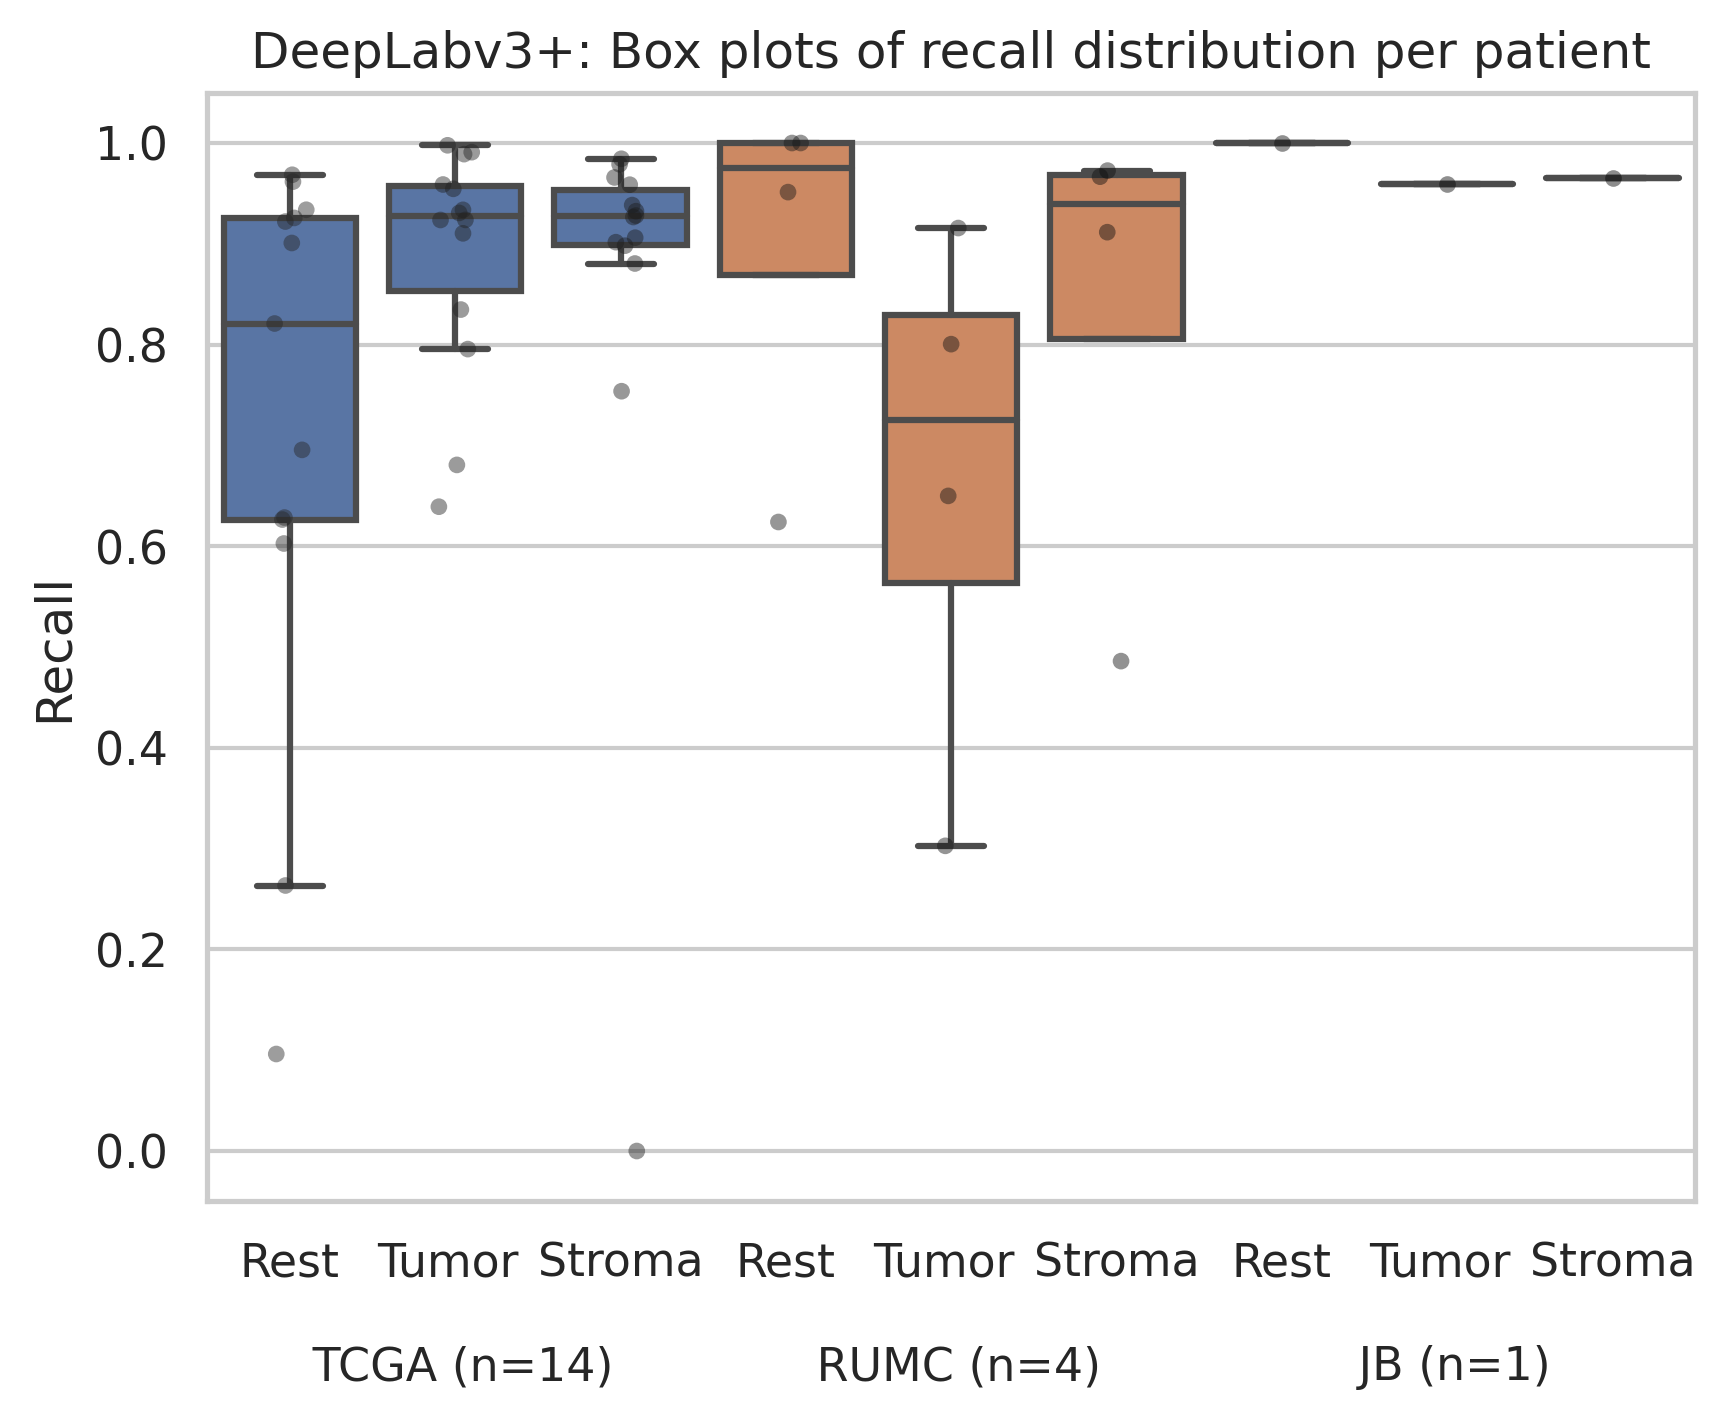
\includegraphics[width=.5\linewidth]{figures/tissue/deeplabv3+_recall_patient_wsirois.png}

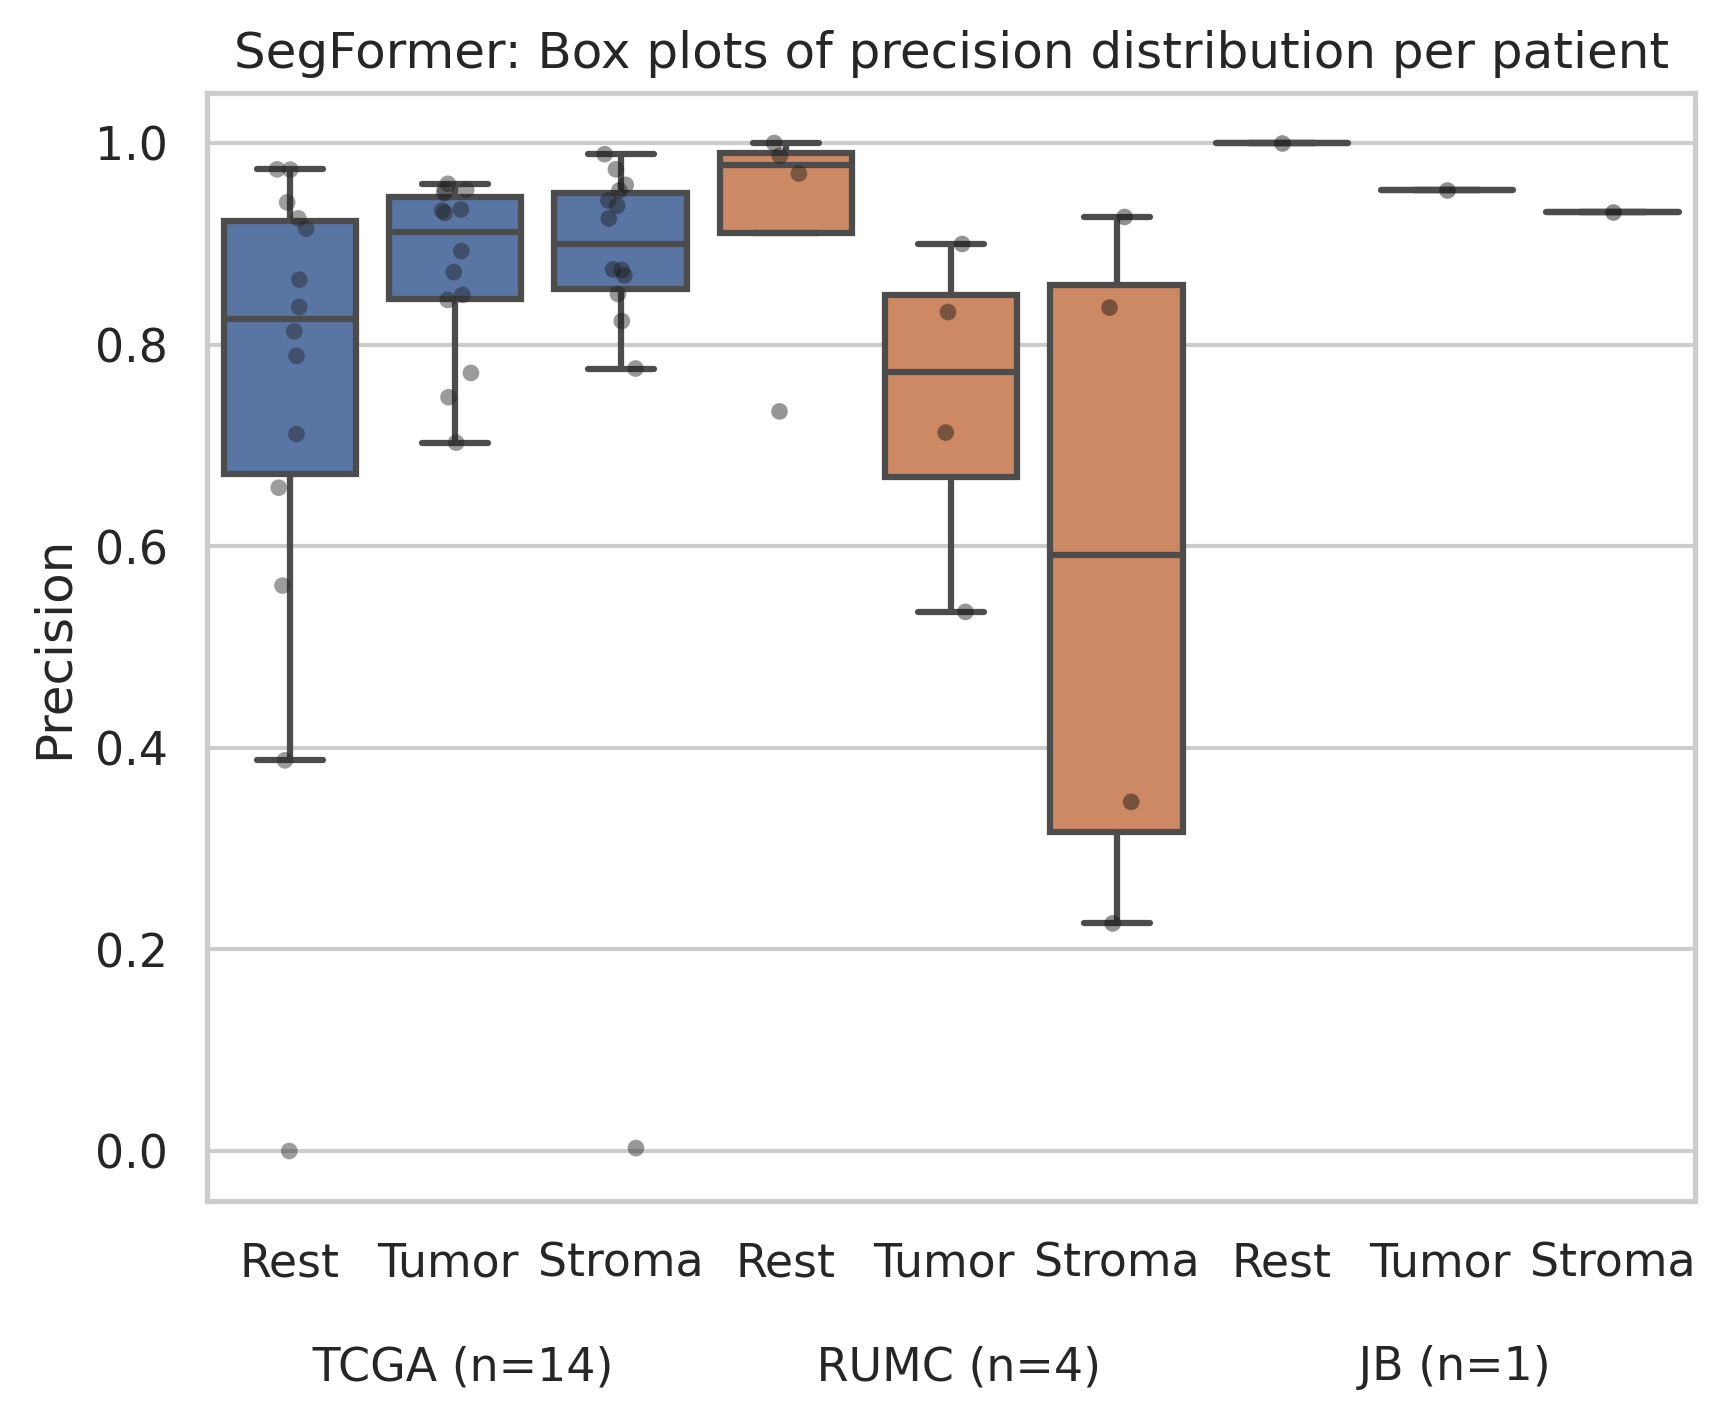
\includegraphics[width=.5\linewidth]{figures/tissue/segformer_prec_patient_wsirois.png}
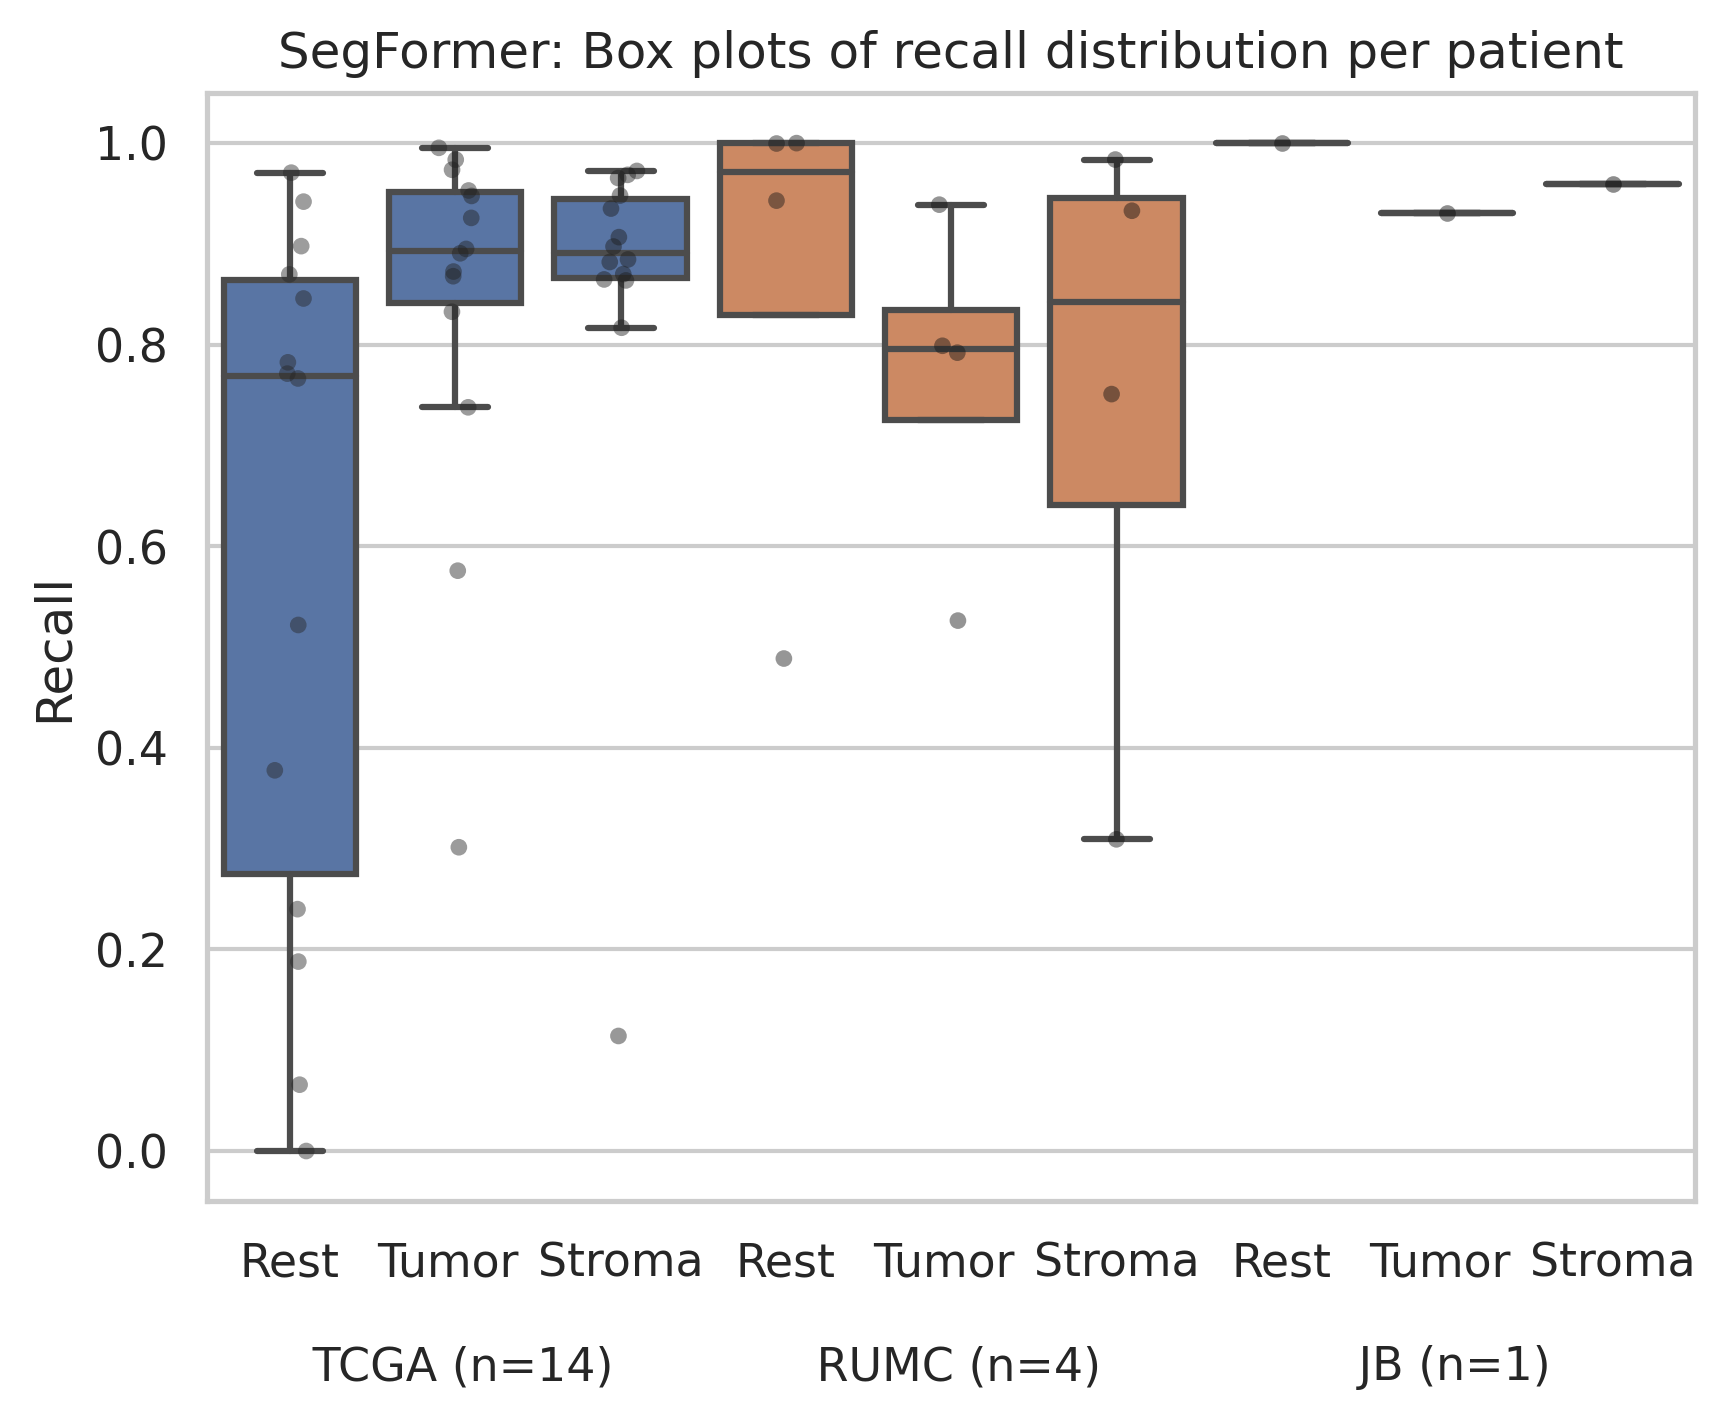
\includegraphics[width=.5\linewidth]{figures/tissue/segformer_recall_patient_wsirois.png}

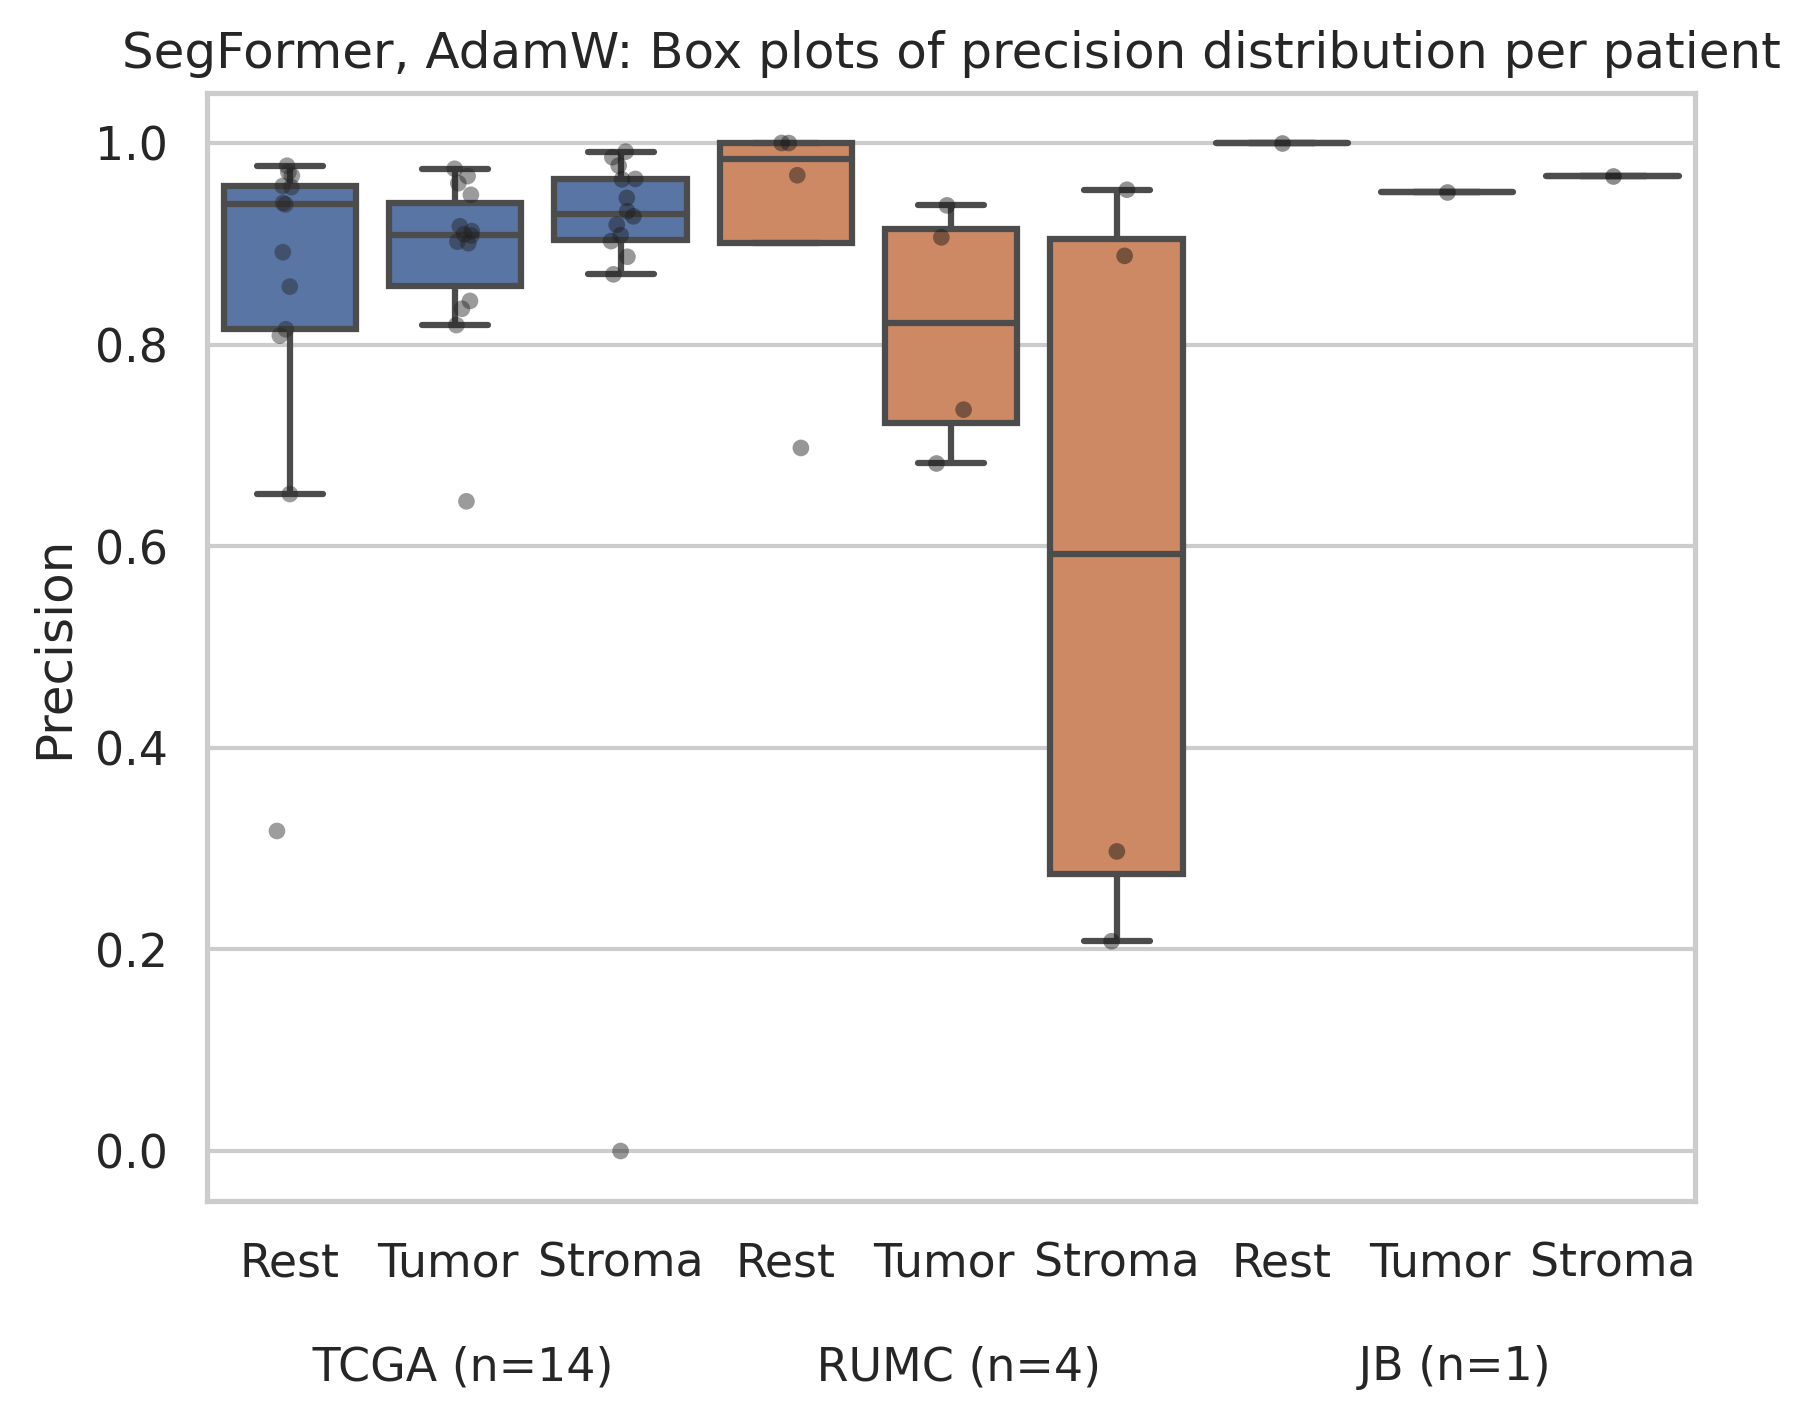
\includegraphics[width=.5\linewidth]{figures/tissue/segformer,_adamw_prec_patient_wsirois.png}
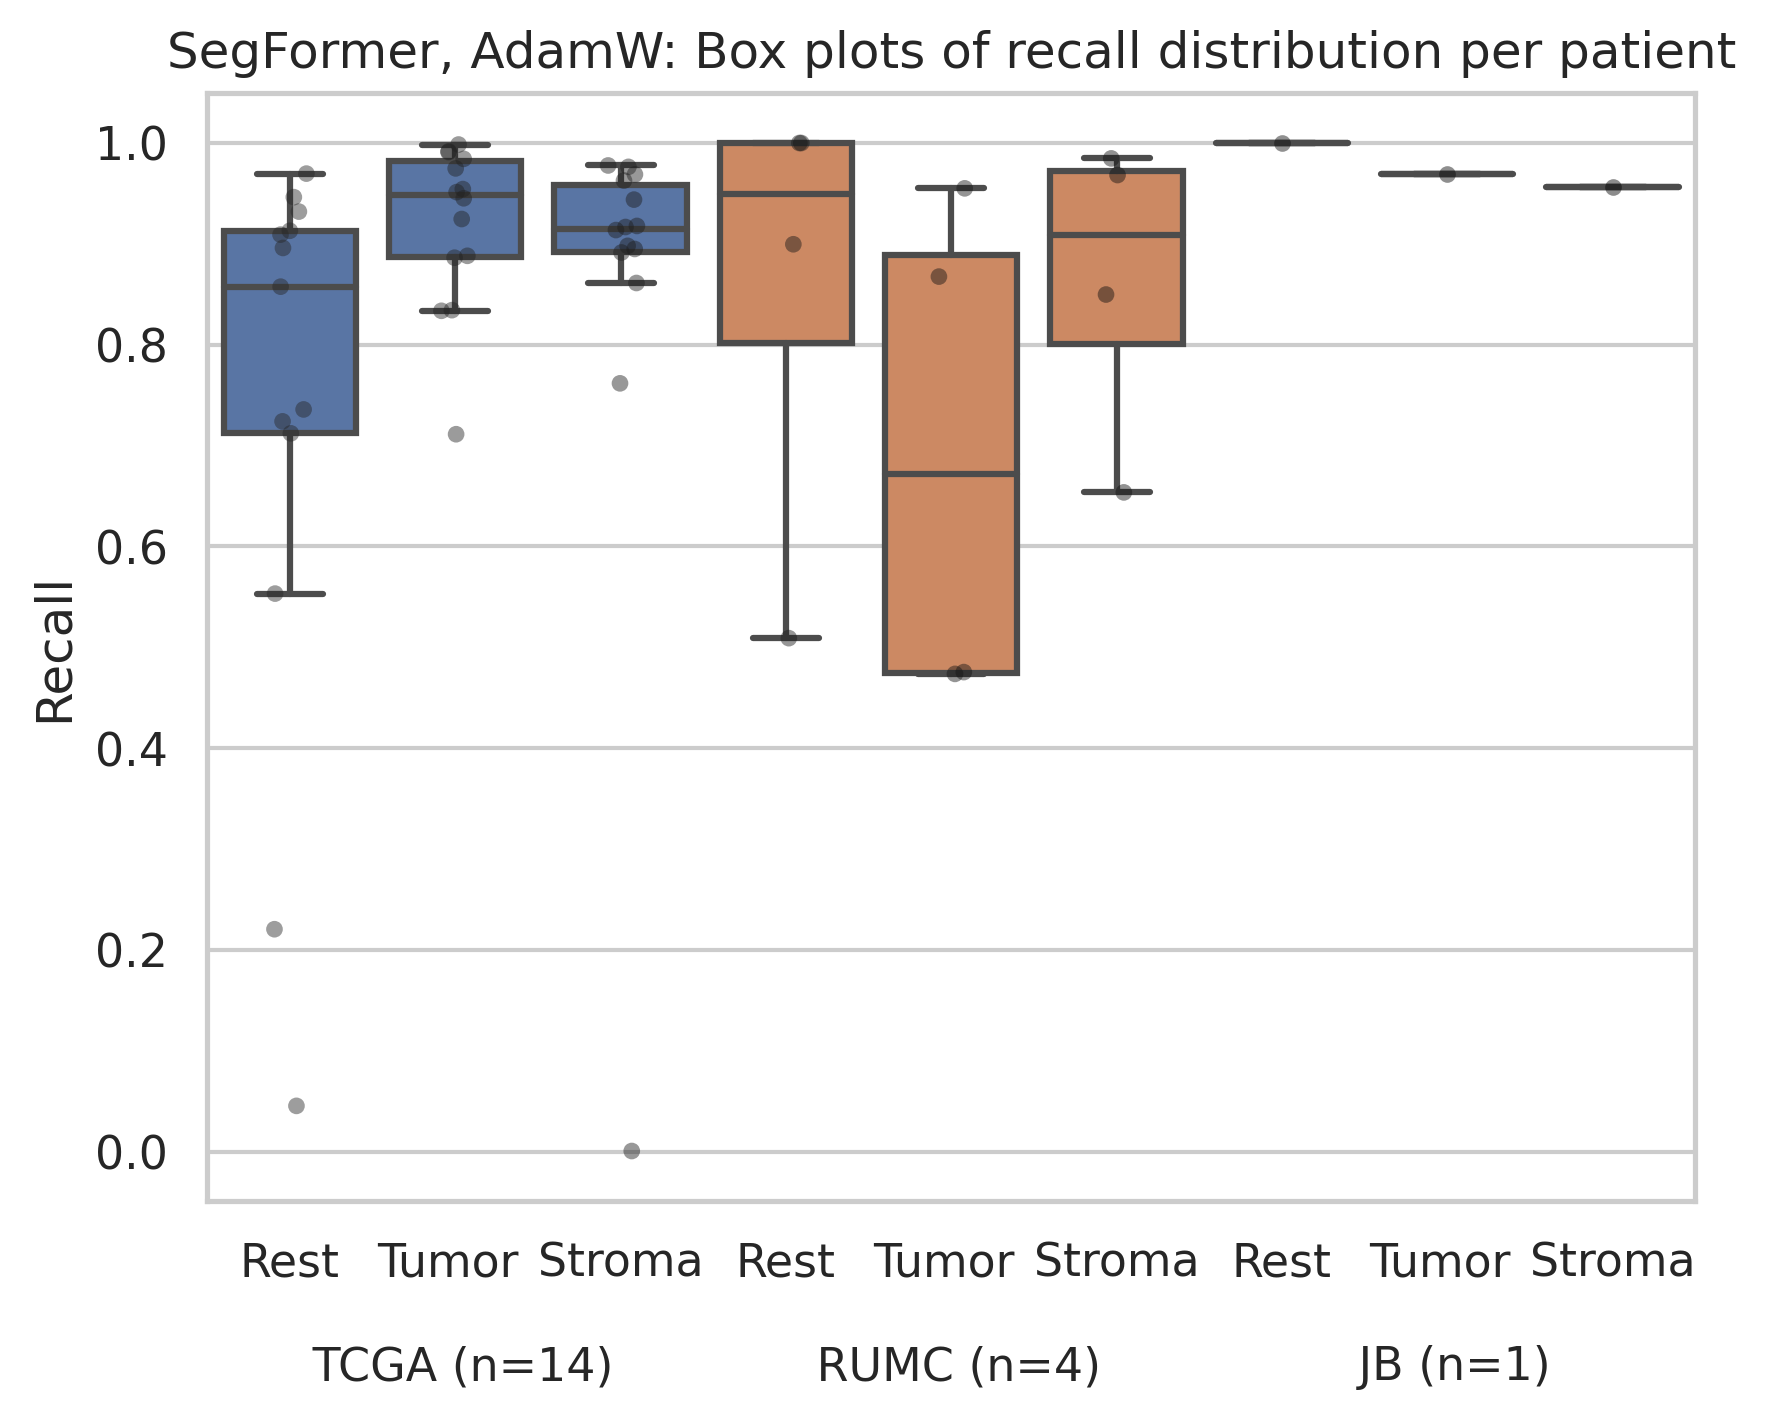
\includegraphics[width=.5\linewidth]{figures/tissue/segformer,_adamw_recall_patient_wsirois.png}

\caption{EXAMPLES for TILs prediction models. A lot of test comming up here.}
\label{fig:figure3}
\end{figure}

\chapter{Figures}
\section{Example 1}
\cmark
\section{Example 2}
\xmark